%\documentstyle[epsf,twocolumn]{jarticle}       %LaTeX2.09仕様
\documentclass[twocolumn]{jarticle}     %pLaTeX2e仕様

%\usepackage[backend=bibtex, style=numeric]{biblatex}
%\addbibresource{sankou.bib}
%%%%%%%%%%%%%%%%%%%%%%%%%%%%%%%%%%%%%%%%%%%%%%%%%%%%%%%%%%%%%%
%%
%%  基本 バージョン
%%
%%%%%%%%%%%%%%%%%%%%%%%%%%%%%%%%%%%%%%%%%%%%%%%%%%%%%%%%%%%%%%%%
\setlength{\topmargin}{-45pt}
%\setlength{\oddsidemargin}{0cm}
\setlength{\oddsidemargin}{-7.5mm}
%\setlength{\evensidemargin}{0cm}
\setlength{\textheight}{24.1cm}
%setlength{\textheight}{25cm}
\setlength{\textwidth}{17.4cm}
%\setlength{\textwidth}{172mm}
\setlength{\columnsep}{11mm}

\setlength{\intextsep}{8pt}
\setlength{\textfloatsep}{8pt}
\setlength{\floatsep}{1pt}

\kanjiskip=.07zw plus.5pt minus.5pt



%【節がかわるごとに(1.1)(1.2) …(2.1)(2.2)と数式番号をつけるとき】
%\makeatletter
%\renewcommand{\theequation}{%
%\thesection.\arabic{equation}} %\@addtoreset{equation}{section}
%\makeatother

%\renewcommand{\arraystretch}{0.95} 行間の設定

\usepackage[dvipdfmx]{graphicx}   %pLaTeX2e仕様(\documentstyle ->\documentclass)
\usepackage{scalefnt}
\usepackage{bm}
\usepackage{here}
\usepackage{url}
\usepackage{amsmath}
\usepackage{amsfonts}
\usepackage[subrefformat=parens]{subcaption}
\captionsetup{compatibility=false}
%%%%%%%%%%%%%%%%%%%%%%%%%%%%%%%%%%%%%%%%%%%%%%%%%%%%%%%%
\usepackage{comment}
\usepackage{subcaption}
\usepackage{multirow}
\usepackage{nidanfloat}
\usepackage[dvipdfmx]{hyperref}

\usepackage[normalem]{ulem}
\useunder{\uline}{\ul}{}

\begin{document}

\twocolumn[
\noindent
\hspace{1em}

令和2年5月13日(水) ゼミ資料
\hfill
\ \ B4 高山 裕成

\vspace{2mm}
\hrule
\begin{center}
{\Large  進捗報告}
\end{center}
\hrule
\vspace{3mm}
]

\section{あらすじ}
テーマは「自然言語処理と深層学習に基づいた 4 コマ漫画のセリフの感情推定」
前回からのタスクは BERT\cite{BERT} の fine-tuning バグ探しとやり直し, 及び作成した Doc2Vec モデルとの比較.

% \footnotesize
\section{進捗}

\begin{itemize}
  \item BERT の fine-tuning やり直し, 及び作成した Doc2Vec モデルとの比較
\end{itemize}

\section{BERT fine-tuning}

\subsection{実装の手直し}
先週, 実装したものにおいて, optuna でハイパーパラメータを最適化する際に, ネットワークのパラメータが引き継がれていたままトライアルが進んでいたので, Train 関数
が呼ばれるたびにネットワークを宣言することで解決した.

\subsection{optuna 目的関数}
検証用データセットにおける正例の F1値 が最大を取るときの値を, そのトライアルの評価値とし, この評価値が最大となるトライアルにおけるハイパーパラメータを探索結果とした.
ハイパーパラメータをチューニングしたのちに, その値でネットワークを学習させ, 検証用データセットにおける正例の F1値 が最大となるエポックを採用モデルとし, テストデータセットを用いて性能を確かめた.

\section{実験設定}
本実験では, 各タッチについて感情推定を行った.
本実験で使用するデータセットは全 7 種類の感情ラベル(ニュートラル, 驚愕, 喜楽, 恐怖, 悲哀, 憤怒, 嫌悪)
を持っているが, データ数と解析の難しさの問題から, 今回は喜楽のみを正例, その他を負例とする 2 クラスに分類した.

訓練用及び検証用データは各タッチの前半 1 話から 5 話までの拡張されたセリフを用い, 訓練用データの内 20 \% をサンプリングして検証用データとした.
評価用データは後半 6 話から 10 話におけるオリジナルのセリフのみを用いた.

分散表現化には以下の 4 パターンを用い, 識別器としては Doc2Vec においては 3 層 MLP, BERT では 1 層の全結合層を用いた. MLP のパラメータを図\ref{table:net_para}に示す.
\begin{itemize}
  \item Doc2Vec (manga109)
  \item Doc2Vec (wiki)
  \item Doc2Vec (manga109 + wiki)
  \item BERT pretrained model\footnote{http://nlp.ist.i.kyoto-u.ac.jp}
\end{itemize}

入力は 1 つのセリフ文, 出力は感情ラベル(0:'喜楽', 1:'その他')であり, またクラス重みとしては訓練用データセットにおける正規化されたラベル数逆比を用いた.
実行ソースコードは ``1g-hub/takayama/src/ex\_2020\_5\_12.py" 及び ``ex\_2020\_5\_12\_2.py" である.

\begin{table}
\caption{MLP パラメータ}
\label{table:net_para}
\centering
\begin{tabular}{|c||c|}
\hline
& MLP \\ \hline
(in,hidden,out) & (300,30,2)\\ \hline
dropout rate & 0.5 \\ \hline
activation function & tanh\\ \hline
\end{tabular}
\end{table}


学習パラメータを表\ref{table:ex_para} に示す. 学習率は optuna によって最適化されたものを用いた.

\begin{table}
\caption{学習パラメータ}
\label{table:ex_para}
\centering
\begin{tabular}{|c||c|c|}
\hline
& \multicolumn{2}{|c|}{実験} \\ \hline
epoch & \multicolumn{2}{|c|}{200}  \\ \hline
batch size & \multicolumn{2}{|c|}{16} \\ \hline
loss function & \multicolumn{2}{|c|}{Cross Entropy Loss} \\ \hline
optimizer & \multicolumn{2}{|c|}{Adam} \\ \hline
\end{tabular}
\end{table}


\section{結果}
実験の結果を表\ref{tab:result} に示す.
表より, BERT fine-tuning は正例に偏るか負例に偏ってしまっており, どの d2v モデルよりも劣った結果となった. またギャグタッチ以外では loss の減少は見られず, 学習が進んでいるとは言えなかった. この原因としては, 全結合層だけでは表現しきれなかった可能性や optuna のパラメータ候補の範囲が不適切である可能性等が考えられる. d2v モデルの比較では平均は manga109 より wiki が若干勝っているといえるがタッチごとに見ると一概にそうとは言えない. manga109 + wiki で性能が上がったタッチもあったが, こちらも一概には言えない.

計算時間は BERT が 約 15 sec / epoch, d2v が 約 1.5 sec / epoch であった.

\begin{table*}[!b]
\begin{center}
\caption{result}
\scalebox{0.65}{
\begin{tabular}{lccccccccccccccc|ccc}
\hline
\multicolumn{1}{c}{\multirow{2}{*}{model}} & \multicolumn{3}{c}{ギャグ} & \multicolumn{3}{c}{少女漫画} & \multicolumn{3}{c}{少年漫画} & \multicolumn{3}{c}{青年漫画} & \multicolumn{3}{c|}{萌え系} & \multicolumn{3}{c}{5タッチ平均} \\
\multicolumn{1}{c}{} & \multicolumn{1}{c}{Acc} & \multicolumn{1}{c}{Recall} & \multicolumn{1}{c}{F1} & \multicolumn{1}{c}{Acc} & \multicolumn{1}{c}{Recall} & \multicolumn{1}{c}{F1} & \multicolumn{1}{c}{Acc} & \multicolumn{1}{c}{Recall} & \multicolumn{1}{c}{F1} & \multicolumn{1}{c}{Acc} & \multicolumn{1}{c}{Recall} & \multicolumn{1}{c}{F1} & \multicolumn{1}{c}{Acc} & \multicolumn{1}{c}{Recall} & \multicolumn{1}{c|}{F1} & \multicolumn{1}{c}{Acc} & \multicolumn{1}{c}{Recall} & \multicolumn{1}{c}{F1} \\ \hline
d2v (manga109) & 0.652 & 0.300 & {\ul 0.207} & 0.537 & 0.632 & 0.608 & 0.625 & 0.667 & 0.400 & 0.662 & 0.357 & 0.312 & 0.563 & 0.364 & 0.364 & 0.608 & 0.464 & 0.378 \\
d2v (wiki) & 0.652 & 0.200 & 0.148 & 0.433 & 0.447 & 0.472 & 0.781 & 0.500 & {\ul 0.462} & 0.815 & 0.643 & {\ul 0.600} & 0.531 & 0.409 & 0.375 & 0.642 & 0.440 & {\ul 0.411} \\
d2v (manga109 + wiki) & 0.621 & 0.200 & 0.138 & 0.612 & 0.579 & {\ul 0.629} & 0.750 & 0.250 & 0.273 & 0.708 & 0.429 & 0.387 & 0.531 & 0.455 & 0.400 & {\ul 0.644} & 0.382 & 0.365 \\
BERT fine-tuning & 0.803 & 0.000 & 0.000 & 0.433 & 0.000 & 0.000 & 0.188 & 1.000 & 0.316 & 0.215 & 1.000 & 0.354 & 0.344 & 1.000 & {\ul 0.512} & 0.397 & 0.600 & 0.236 \\ \hline
ベースライン & \multicolumn{1}{c}{0.85} & \multicolumn{1}{c}{0} & \multicolumn{1}{c}{0} & \multicolumn{1}{c}{0.43} & \multicolumn{1}{c}{0} & \multicolumn{1}{c}{0} & \multicolumn{1}{c}{0.81} & \multicolumn{1}{c}{0} & \multicolumn{1}{c}{0} & \multicolumn{1}{c}{0.78} & \multicolumn{1}{c}{0} & \multicolumn{1}{c}{0} & \multicolumn{1}{c}{0.66} & \multicolumn{1}{c}{0} & \multicolumn{1}{c|}{0} & \multicolumn{1}{c}{0.71} & \multicolumn{1}{c}{0} & \multicolumn{1}{c}{0}
\end{tabular}
\label{tab:result}
}
\end{center}
\end{table*}

\section{今後の実験予定}
\begin{itemize}
  \item 識別器をそろえて再実験.
  \item optuna でのハイパーパラメータの値の範囲や試行回数について考察.
  \item 正例に指定する感情ラベルを変えて実験. (ニュートラル, 驚愕, 喜楽)
  \item 直前 n - 1 文 を考慮した n 文を入力して末尾入力の感情推定をする. モデル図は 図\ref{fig:seq}
\end{itemize}

\begin{figure}[htb]
  \begin{center} %センタリングする
    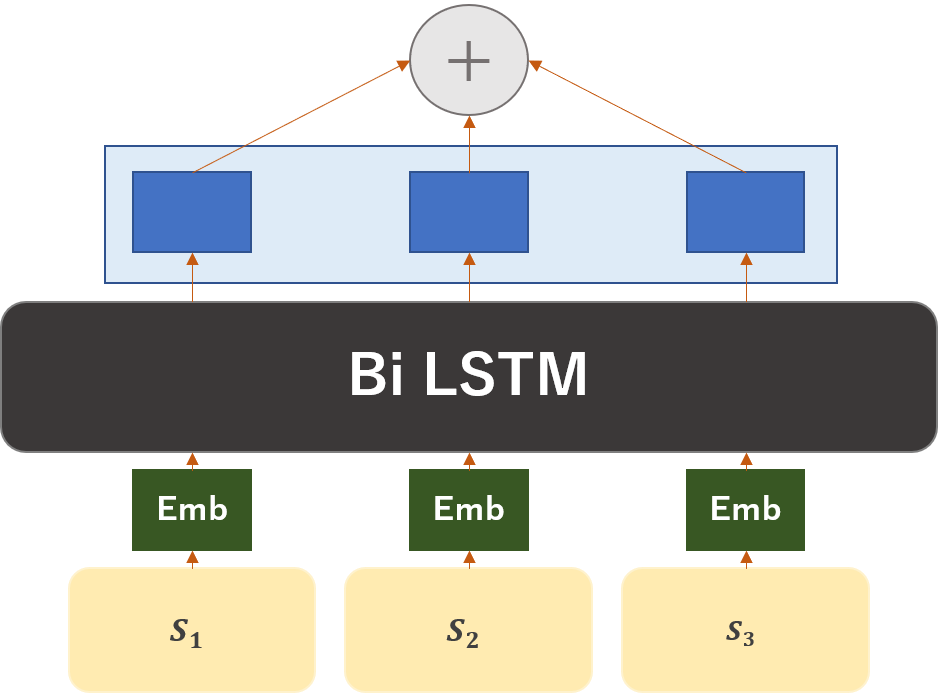
\includegraphics[width=7.0cm]{net.png}
    \caption{seq experiment net} %タイトルをつける
    \label{fig:seq} %ラベルをつけ図の参照を可能にする
  \end{center}
\end{figure}

\section{その他 課題}
\begin{itemize}
  \item 森先生と大工大の上野先生に 30 話まであるらしい追加データをお願いする.
  \item Data Augmentation の手法の改善案.
\end{itemize}


\bibliographystyle{unsrt}
\bibliography{sankou}

\clearpage
\begin{figure*}[h]
  \begin{center} %センタリングする
    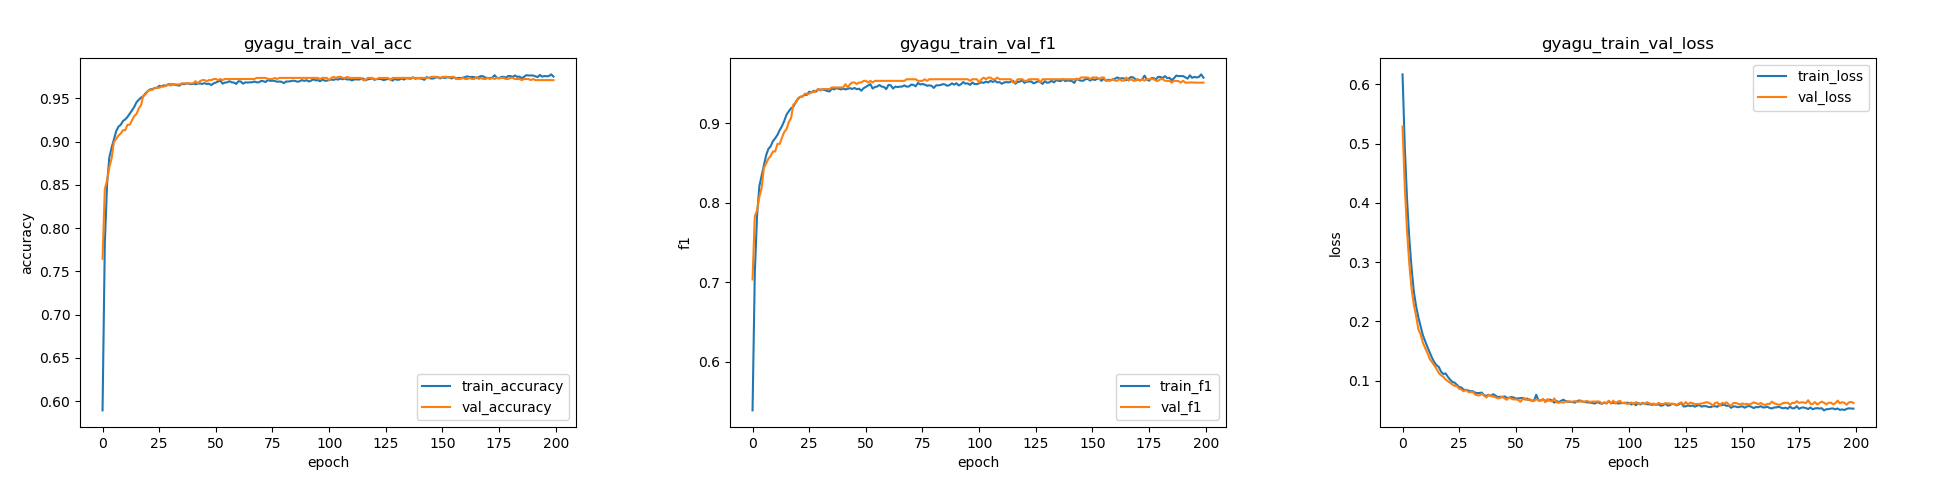
\includegraphics[width=14.0cm]{gyagu_d2v_manga109.png}
    \caption{gyagu\_d2v\_manga109} %タイトルをつける
    \label{fig:gyagu_d2v_manga109} %ラベルをつけ図の参照を可能にする
  \end{center}
\end{figure*}

\begin{figure*}[h]
  \begin{center} %センタリングする
    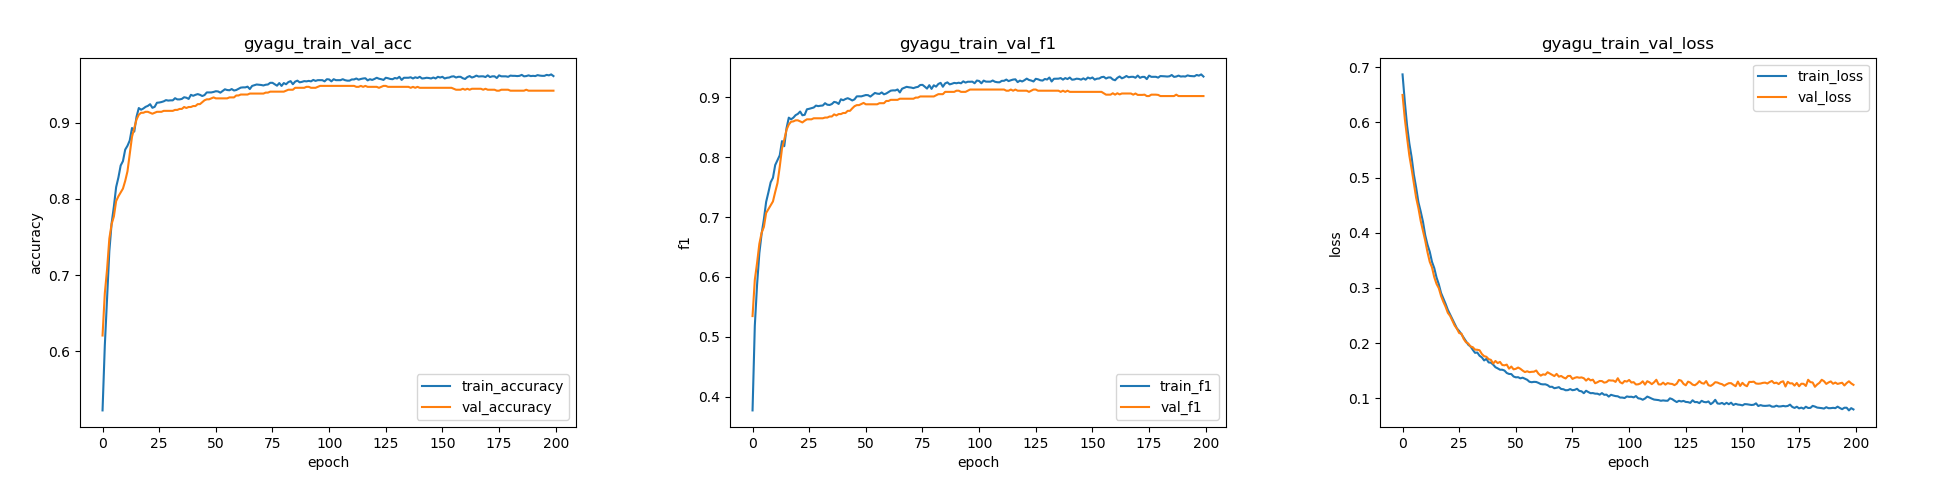
\includegraphics[width=14.0cm]{gyagu_d2v_wiki.png}
    \caption{gyagu\_d2v\_wiki} %タイトルをつける
    \label{fig:gyagu_d2v_wiki} %ラベルをつけ図の参照を可能にする
  \end{center}
\end{figure*}

\begin{figure*}[h]
  \begin{center} %センタリングする
    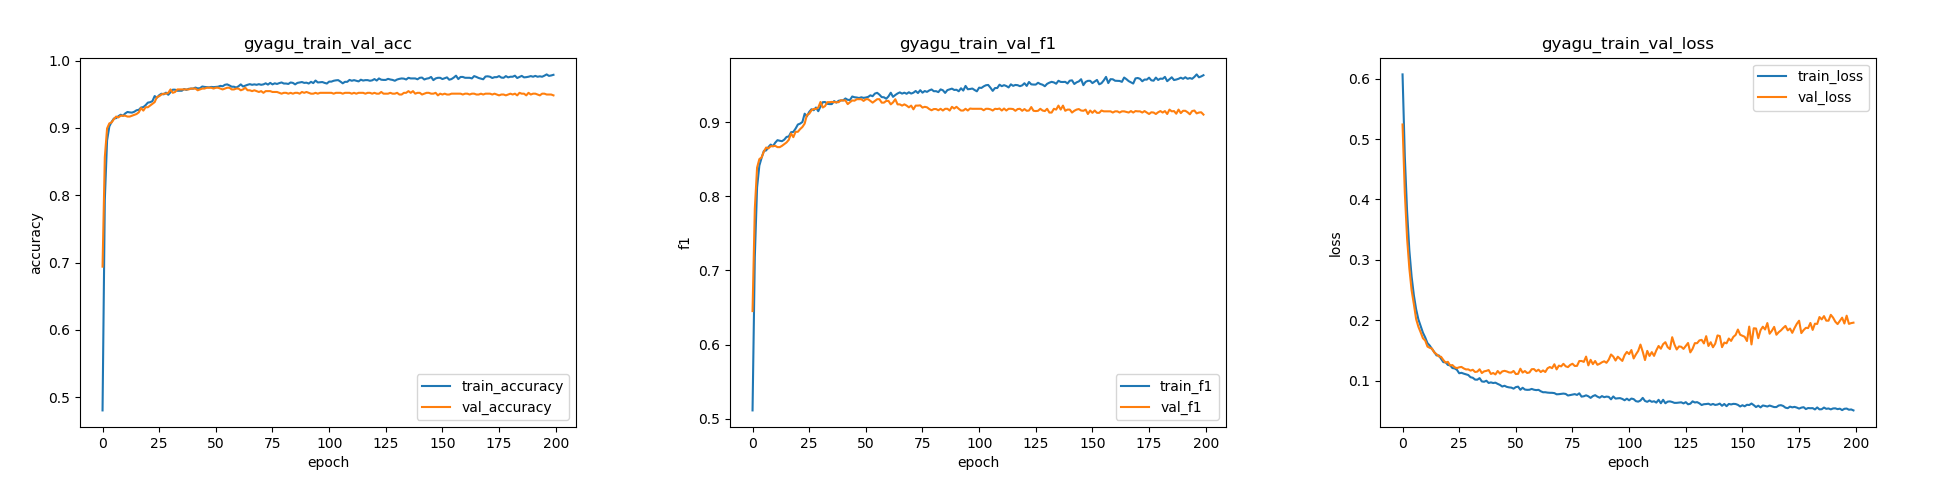
\includegraphics[width=14.0cm]{gyagu_d2v_manga109_wiki.png}
    \caption{gyagu\_d2v\_manga109\_wiki} %タイトルをつける
    \label{fig:gyagu_d2v_manga109_wiki} %ラベルをつけ図の参照を可能にする
  \end{center}
\end{figure*}

\clearpage

\begin{figure*}[h]
  \begin{center} %センタリングする
    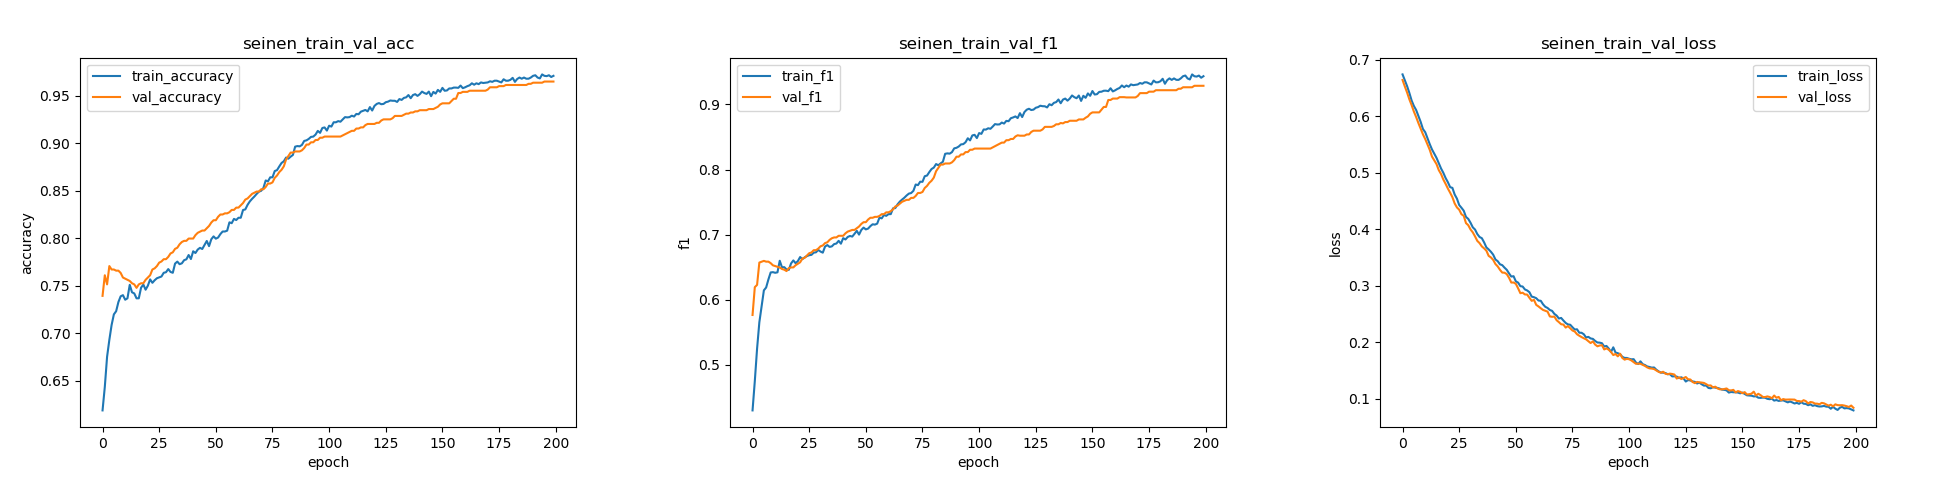
\includegraphics[width=14.0cm]{seinen_manga109.png}
    \caption{seinen\_d2v\_manga109} %タイトルをつける
    \label{fig:seinen_d2v_manga109} %ラベルをつけ図の参照を可能にする
  \end{center}
\end{figure*}

\begin{figure*}[h]
  \begin{center} %センタリングする
    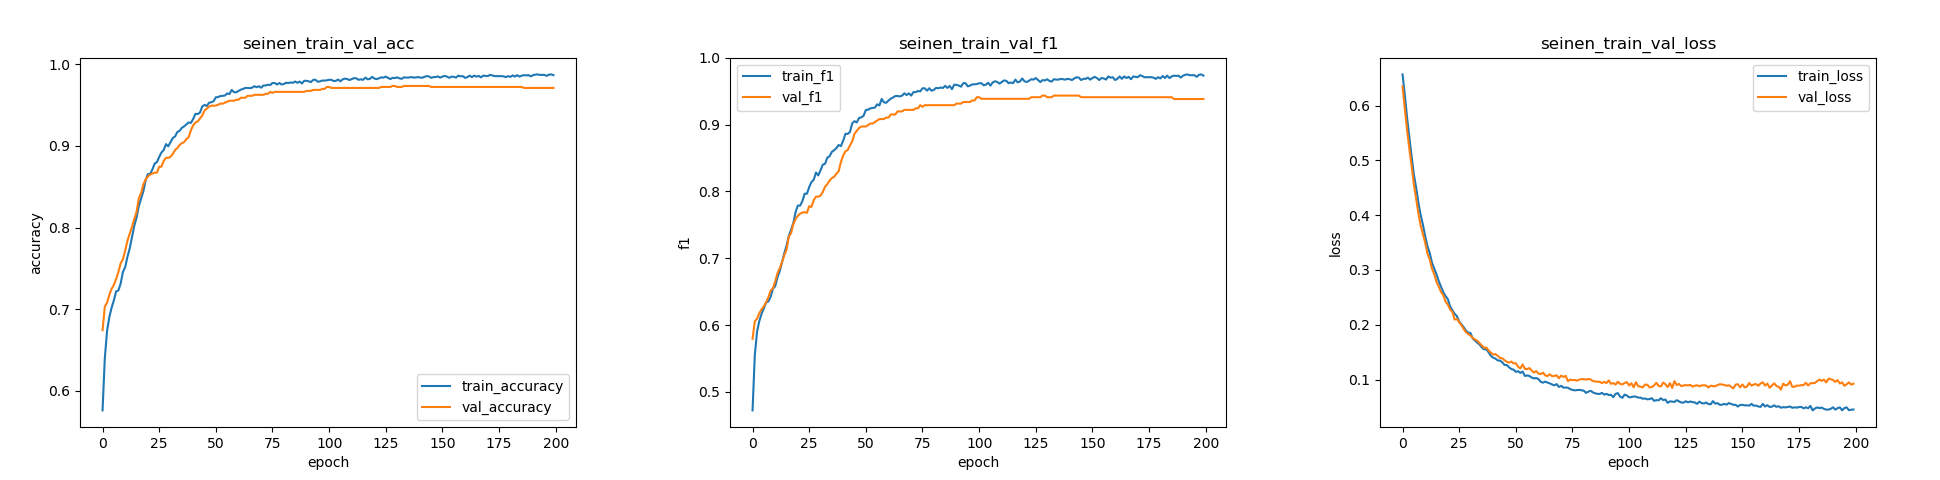
\includegraphics[width=14.0cm]{seinen_wiki.png}
    \caption{seinen\_d2v\_wiki} %タイトルをつける
    \label{fig:seinen_d2v_wiki} %ラベルをつけ図の参照を可能にする
  \end{center}
\end{figure*}

\begin{figure*}[h]
  \begin{center} %センタリングする
    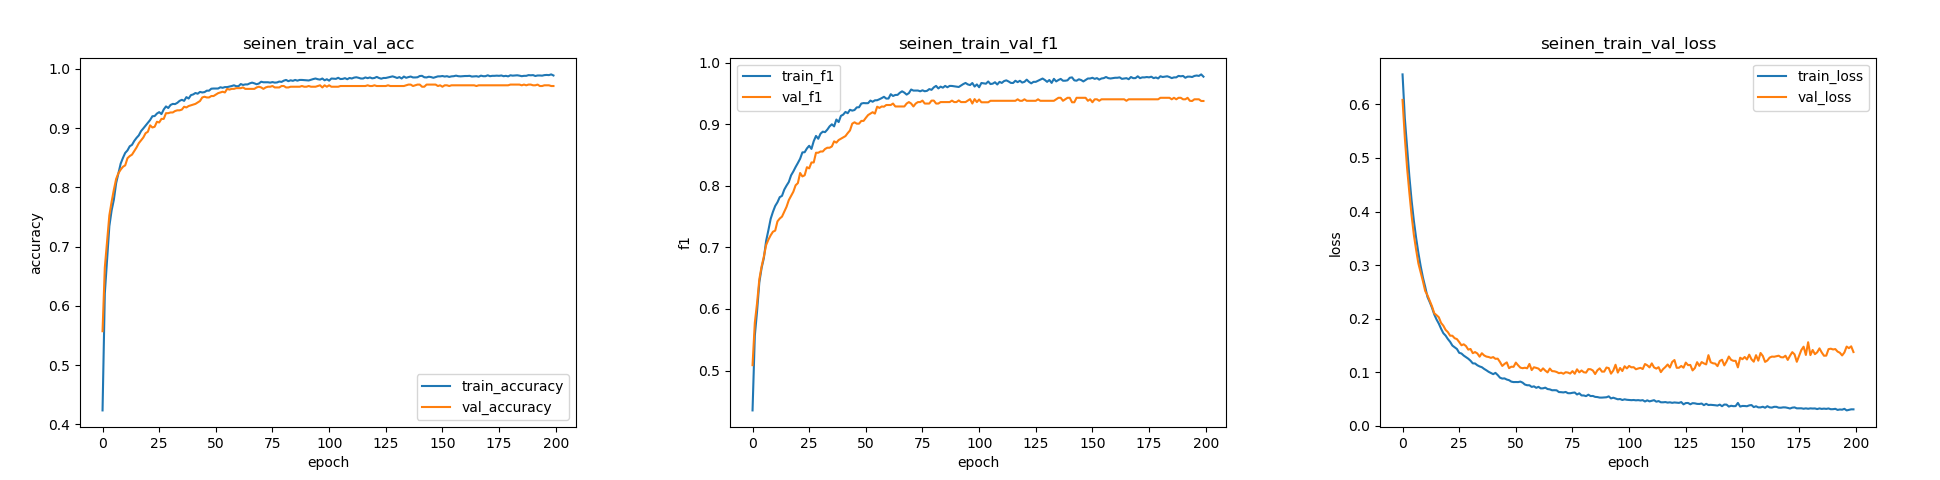
\includegraphics[width=14.0cm]{seinen_manga109_wiki.png}
    \caption{seinen\_d2v\_manga109\_wiki} %タイトルをつける
    \label{fig:seinen_d2v_manga109_wiki} %ラベルをつけ図の参照を可能にする
  \end{center}
\end{figure*}

\clearpage

\begin{figure*}[h]
  \begin{center} %センタリングする
    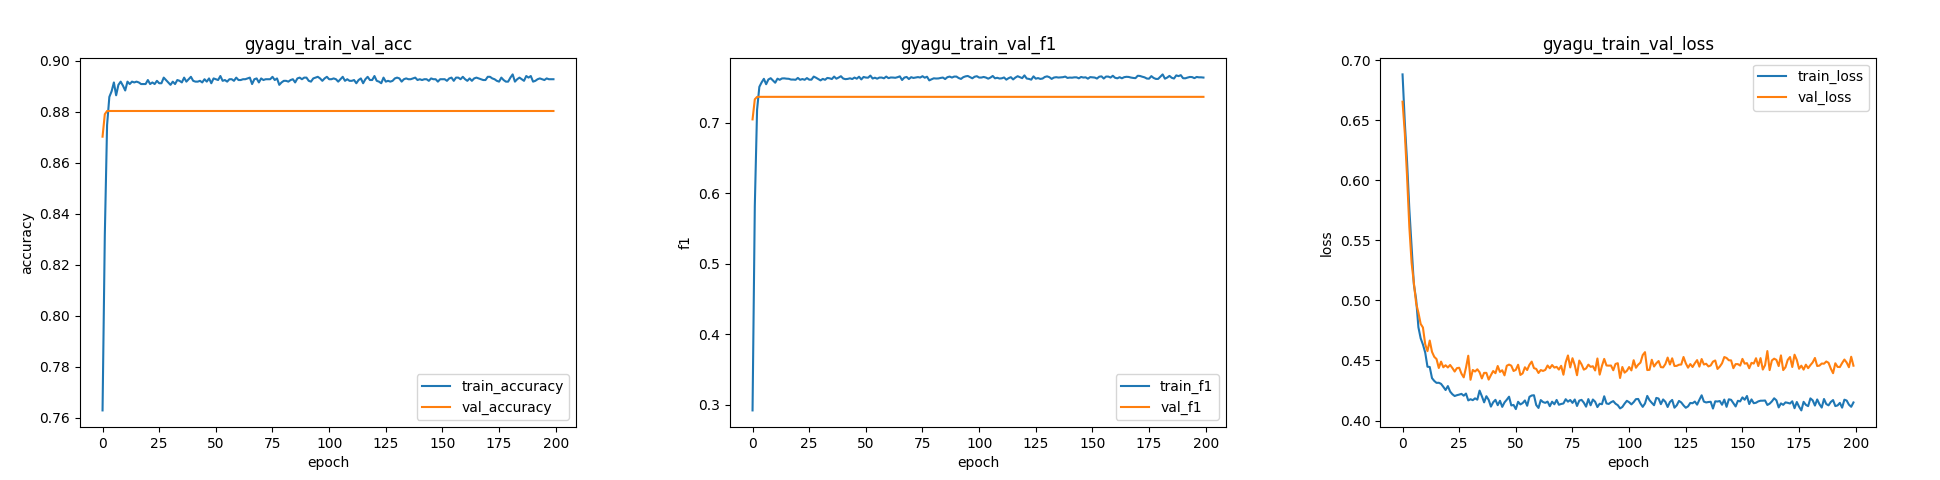
\includegraphics[width=14.0cm]{gyagu_bert.png}
    \caption{gyagu\_bert} %タイトルをつける
    \label{fig:gyagu_bert} %ラベルをつけ図の参照を可能にする
  \end{center}
\end{figure*}

\begin{figure*}[h]
  \begin{center} %センタリングする
    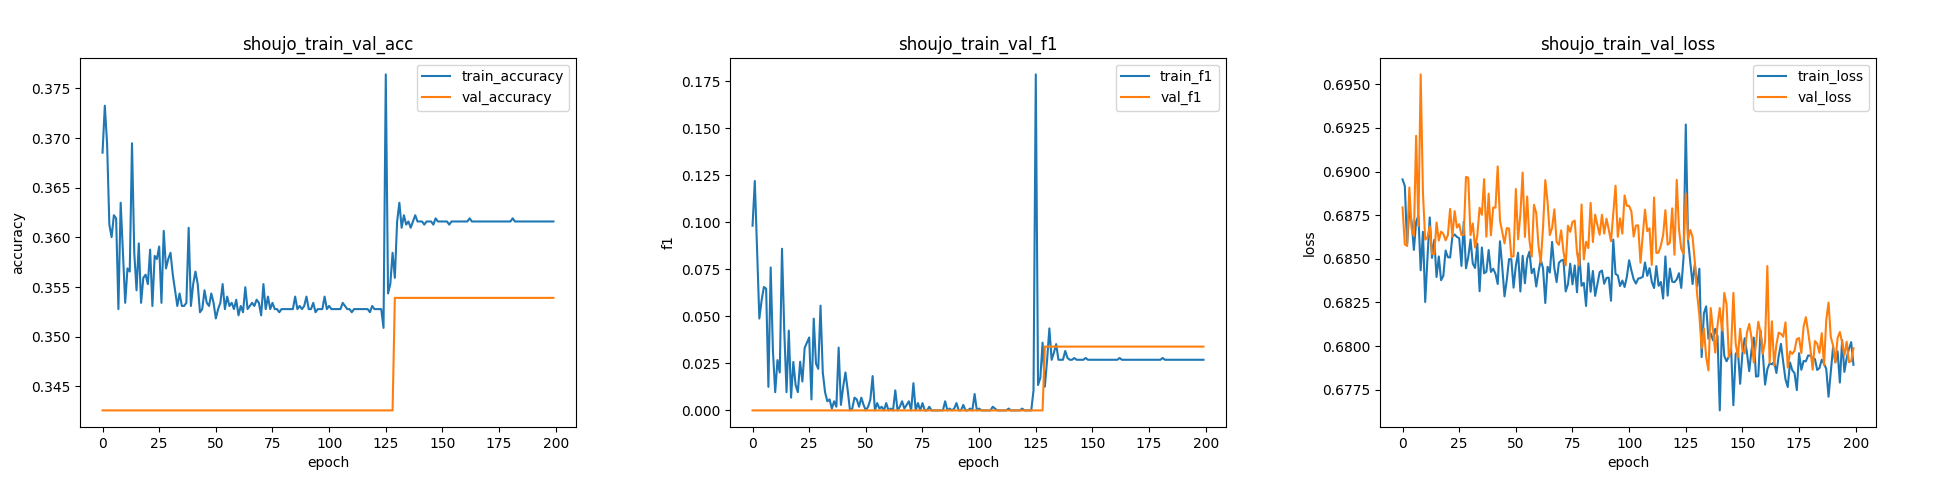
\includegraphics[width=14.0cm]{shoujo_bert.png}
    \caption{shoujo\_bert} %タイトルをつける
    \label{fig:shoujo_bert} %ラベルをつけ図の参照を可能にする
  \end{center}
\end{figure*}

\begin{figure*}[h]
  \begin{center} %センタリングする
    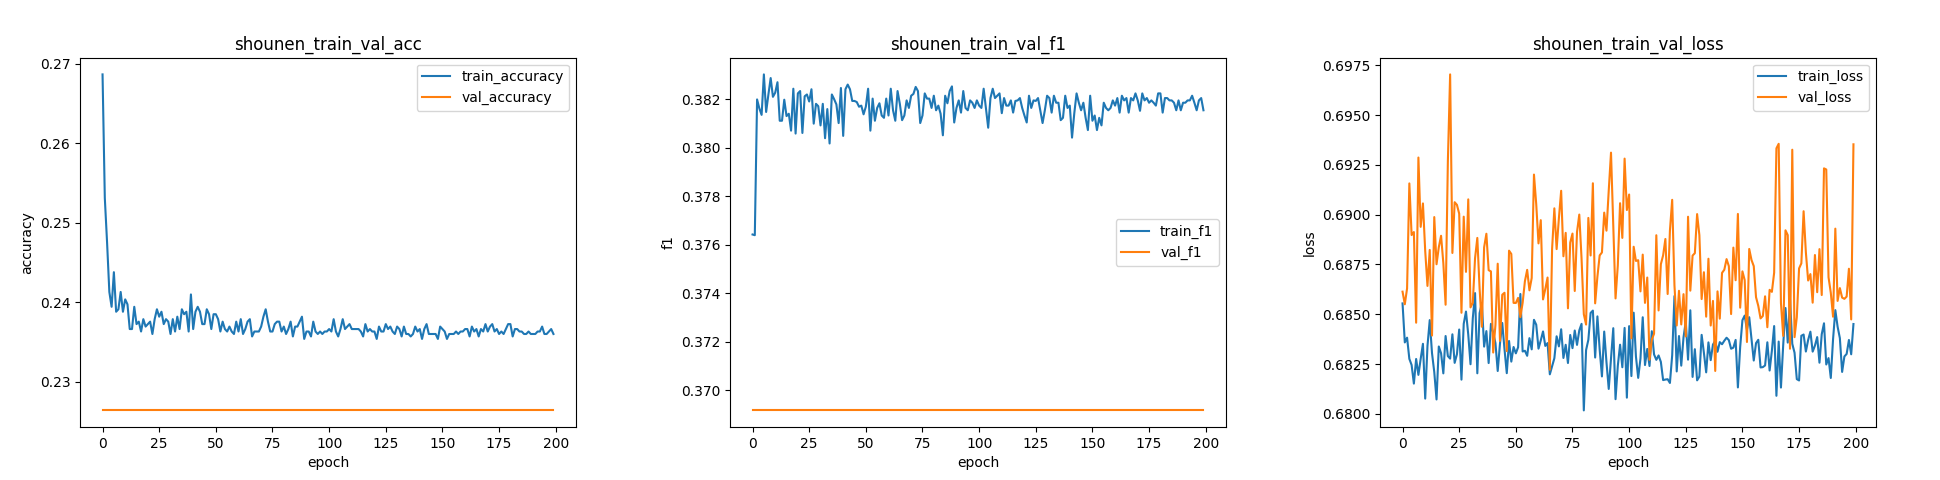
\includegraphics[width=14.0cm]{shounen_bert.png}
    \caption{shounen\_bert} %タイトルをつける
    \label{fig:shounen_bert} %ラベルをつけ図の参照を可能にする
  \end{center}
\end{figure*}

\begin{figure*}[h]
  \begin{center} %センタリングする
    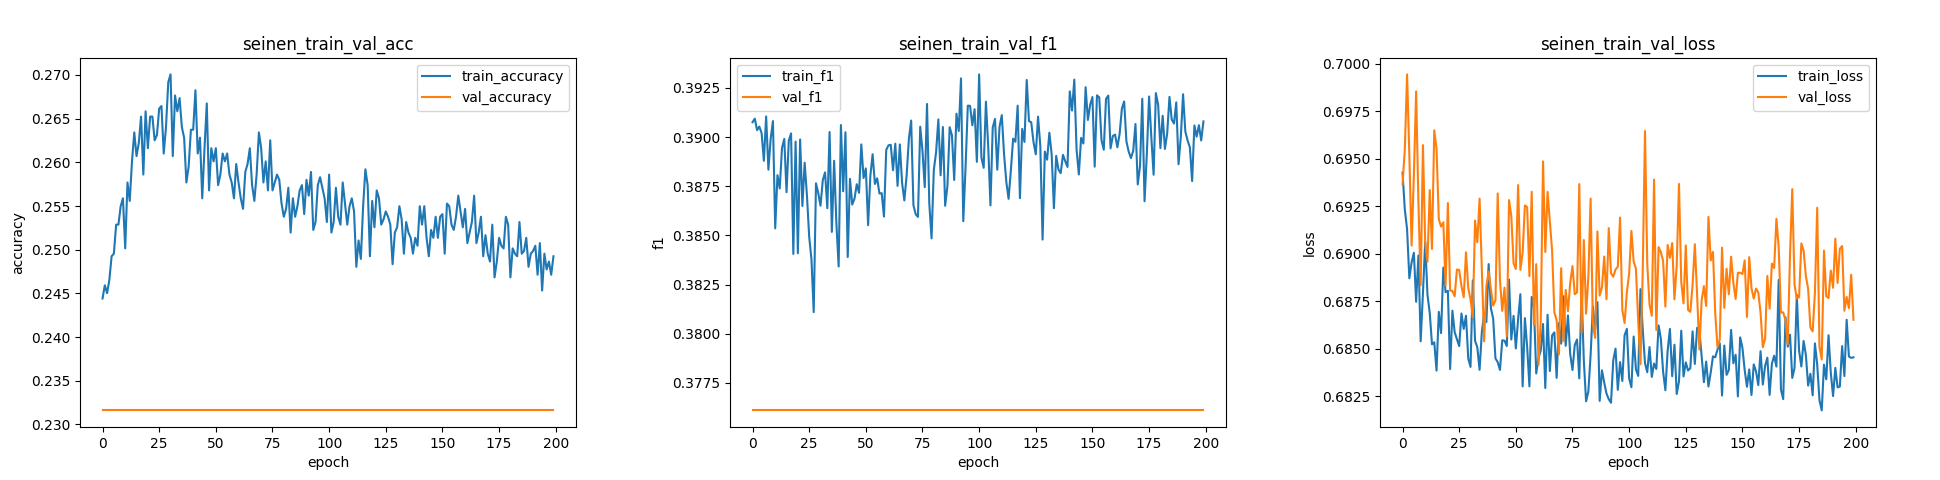
\includegraphics[width=14.0cm]{seinen_bert.png}
    \caption{seinen\_bert} %タイトルをつける
    \label{fig:seinen_bert} %ラベルをつけ図の参照を可能にする
  \end{center}
\end{figure*}

\begin{figure*}[h]
  \begin{center} %センタリングする
    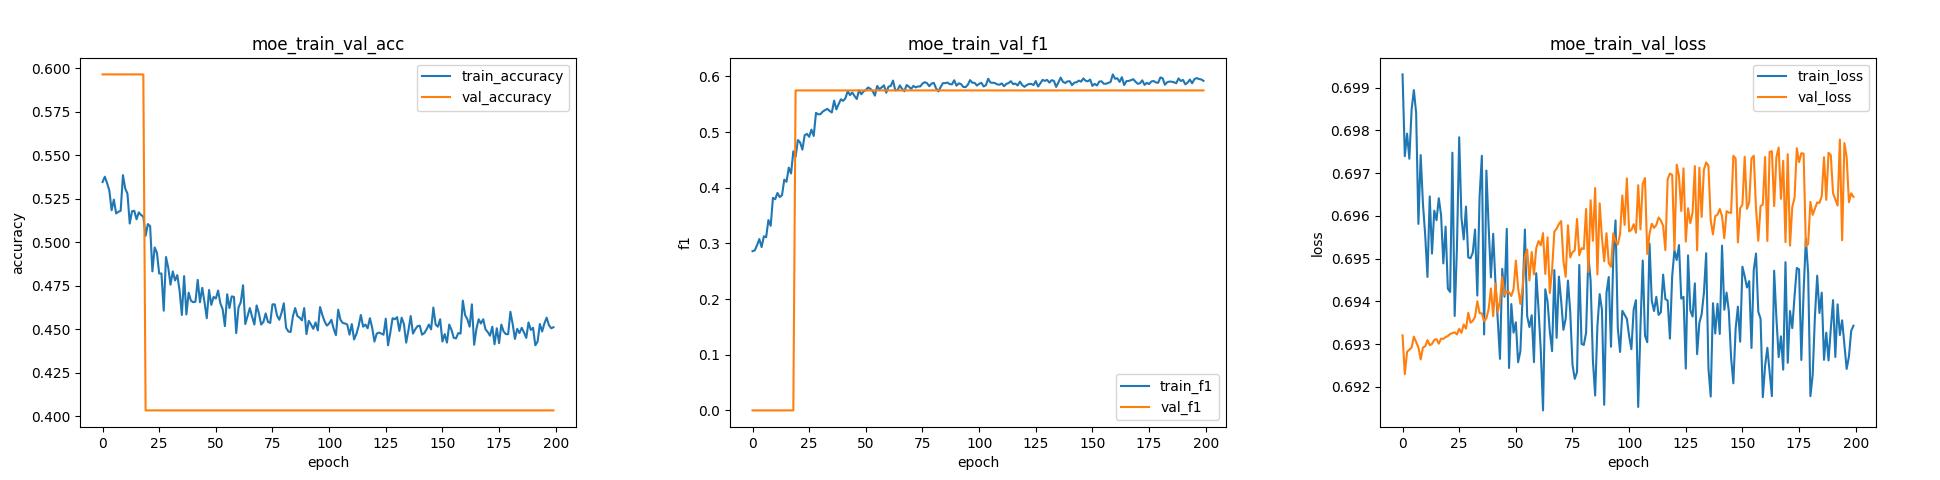
\includegraphics[width=14.0cm]{moe_bert.png}
    \caption{moe\_bert} %タイトルをつける
    \label{fig:moe_bert} %ラベルをつけ図の参照を可能にする
  \end{center}
\end{figure*}
\clearpage
\end{document}
